\chapter{Subsystem: Sensor Housing}

\section{Need for Housing} Our vehicle, being equipped with multiple sensors, including sensors for air particulates, natural gas, petroleum gas, carbon monoxide, carbon dioxide, and hydrogen gas, needs to have an effective way of protecting the sensors from physical elements that could damage them while also ensuring they are in conditions that will allow the sensors to be exposed to the elements they are meant to detect. We decided to house these sensors together into one housing unit. This unit can serve to shield the sensors from any physical interferences.

\section{Materials Used} The material for the housing unit needed to be relatively sturdy to protect the sensors, cheap and easy to machine for economic efficiency, and thermally resistant to protect our sensors from high heat. After researching many materials, Acrylic was decided upon for the material to construct our housing structure.

\begin{table}
\centering
\begin{tabular}{l|r}
Property & Associated Value \\\hline
Thermal Conductivity & 1.3 to 1.5 $\frac{Btu-in}{hr-ft^2-\deg F}$ \\
Melting Temperature & 464 to 473 $\deg$ F \\
Compressive Strength & 14100 to 18000 psi \\
Tensile Strength & 5420 to 10700 psi \\
\end{tabular}
\caption{\label{tab:Acrylic Properties} The properties of acrylic made available from the UL company \cite{UL}}
\end{table}

Acrylic has relatively low thermal conductivity, meaning it can insulate our sensors effectively, and it's melting temperature is far above the temperature maximum of 250$\deg F$ that we expect our vehicle to be present in. Though we do not expect our unit to be under a great deal of stress, as the most stress our vehicle will be in is under the stress of its own weight, the compressive and tensile strength are both well above the weight of the system. The price of acrylic is relatively cheap compared to other plastics of comprable properties, and it is very easy to machine and assemble through the use of adhesives, which would be an ideal means of assembly, as bolts would be innefective for assembling a relatively small housing unit.

\section{Initial Design}

The first of the questions would be how do we force the air into the housing unit? Though our housing unit is designed to protect our sensors from many of the outside elements, our sensors also must be exposed to air. We decided to use a PWM fan for its speed control and relatively small size. The model we are going to use is the Artic F9 Case fan, which reaches a maximum air flow of 31 $ft^{3}/min$. For our initial design, our team decided to use the fan as an outlet for airflow, pulling air through our housing unit.

The next question facing our design concerned the means by which air could flow over and through our sensors. While our specific air sensors, which measure the concentrations of different harmful gasses in the air simply needed air to flow over them, as shown in (Figure of sensor), our air particulate sensor needed air to rise through a very specific segment, as demonstrated in (Figure of air particulate). Due to this, our housing design needed to account for these means of air flow. (Design Picture shows our design (pre-analysis) that we came up with in order to accommodate those needs. Note that there are two main inlet holes, one on the front of the unit, and one on the underside. The front inlet was designed to be the major inlet of air to fill  our housing unit. Our bottom hole was designed specifically to intake air, pushing air directly through the air particulate sensor.

\begin{figure}[H]
	\centering
	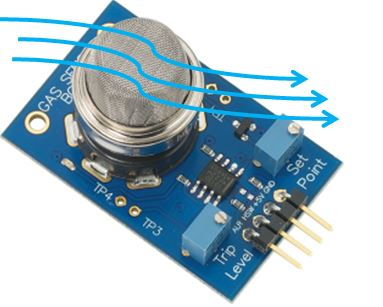
\includegraphics[scale=1]{GasSensorAirflow.jpg}
	\caption{For the gas sensors to work, air must flow over the sensor}
	\label{fig:airflow1}
\end{figure}

\begin{figure}[H]
	\centering
	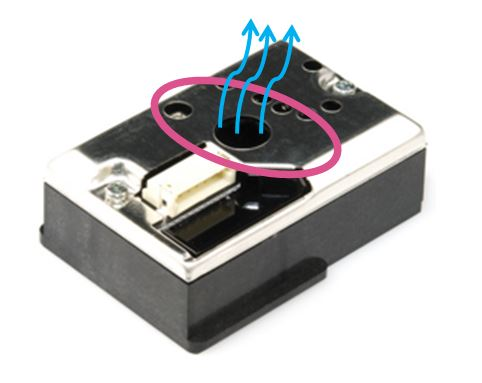
\includegraphics[scale=1]{AirParticulateAirflow.jpg}
	\caption{For the air particulate sensor to work, air must flow through the sensor}
	\label{fig:airflow2}
\end{figure}

The major question we were left with was, will the air flow where we want the air to flow. For this a computational fluid dynamics (CFD) test will be performed on our design.

\section{CFD Analysis and Iterative Work}

Ansys Workbench was used to perform a series of tasks designed to complete a CFD analysis. The first task was to design the internal space of the feature. This means designing a part that would represent only the area inside the housing unit. (Figure of internal Space) shows the design of said part.

After this internal space was designed, a mesh was created around the part using Ansys Workbench. Once the mesh was created and reformatted to be as precise as possible, boundary conditions could be set. No-slip conditions were set on all of the walls of the part. The inlets of the part were set at ambient pressure of 1 atm. The outlet was given a constant outlet velocity, calculated from converting the 31 ft3/min of the fan into m/s by dividing by the area of the fan and converting ft to m, of 2.6058m/s. From there, a streamline map was developed for the system in order to show how successful our design was.

Our streamline map pointed out some key failings of our current design, though we were successful in driving air up the hole dedicated to feeding our air particulate sensor, we were unable to fill the area of the housing unit where most of our other sensors would be placed. Instead of the air filling up the empty space, only a few streamlines reached the center of our housing unit. Instead, many of our streamlines clung to the edge of our design.

\begin{figure}[H]
	\centering
	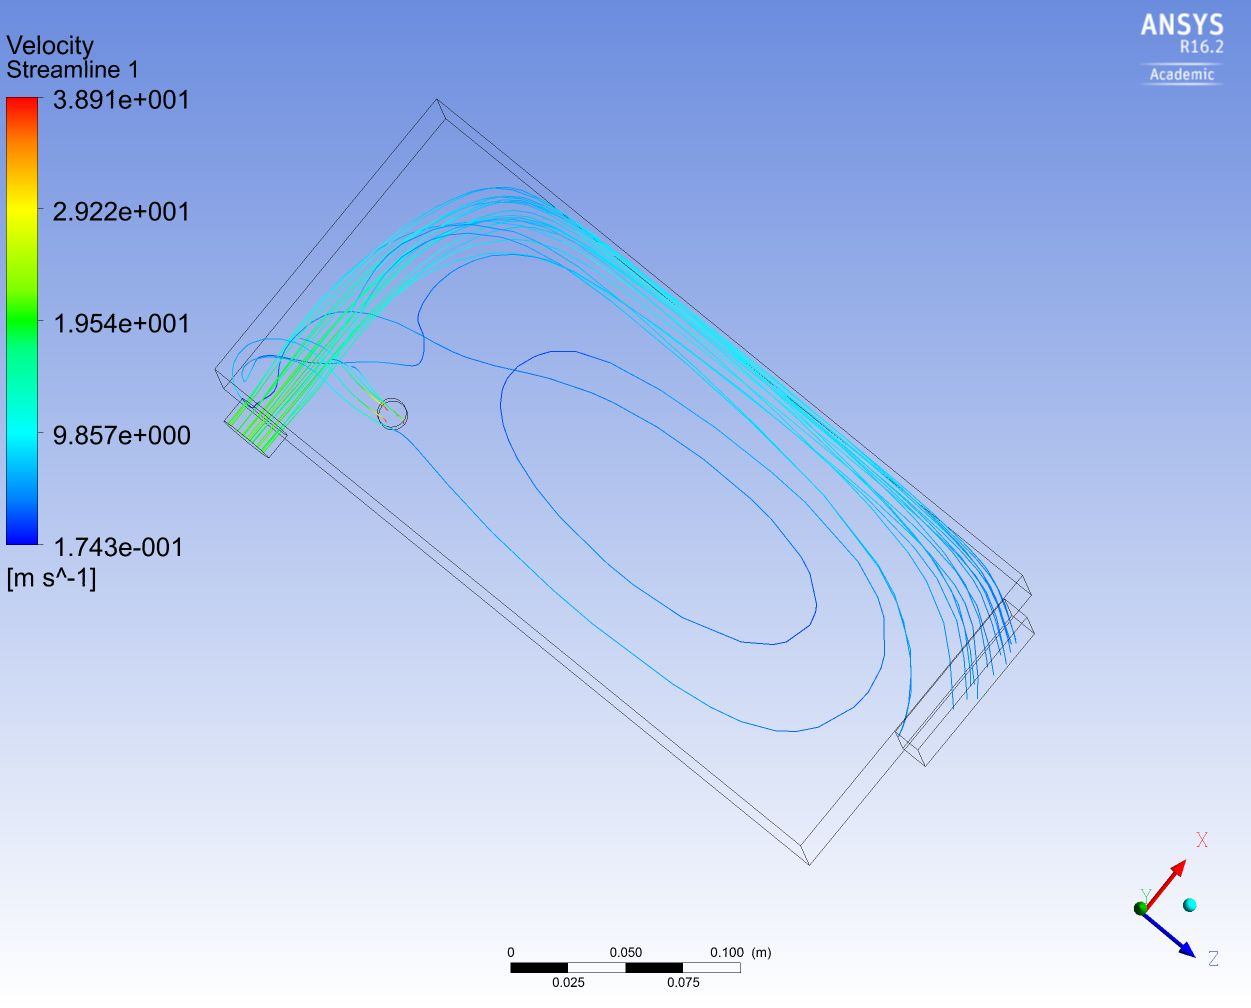
\includegraphics[scale=0.35]{CFDhalf.jpg}
	\caption{CFD streamline analysis for our first design}
	\label{fig:CFD1}
\end{figure}

In our second iteration, we attempted the same tests while adding a second inlet hole on the opposite side of the housing unit to our primary inlet. This was added to push air streams into the streams currently clinging to the wall of our unit in order to send air through the central area of our housing unit, where the gas sensors would most likely be. While this did move air more successfully through our system than the prior design, there were still inconsistencies in the streamlines as vorticies were created as the streams collided.

\begin{figure}[H]
	\centering
	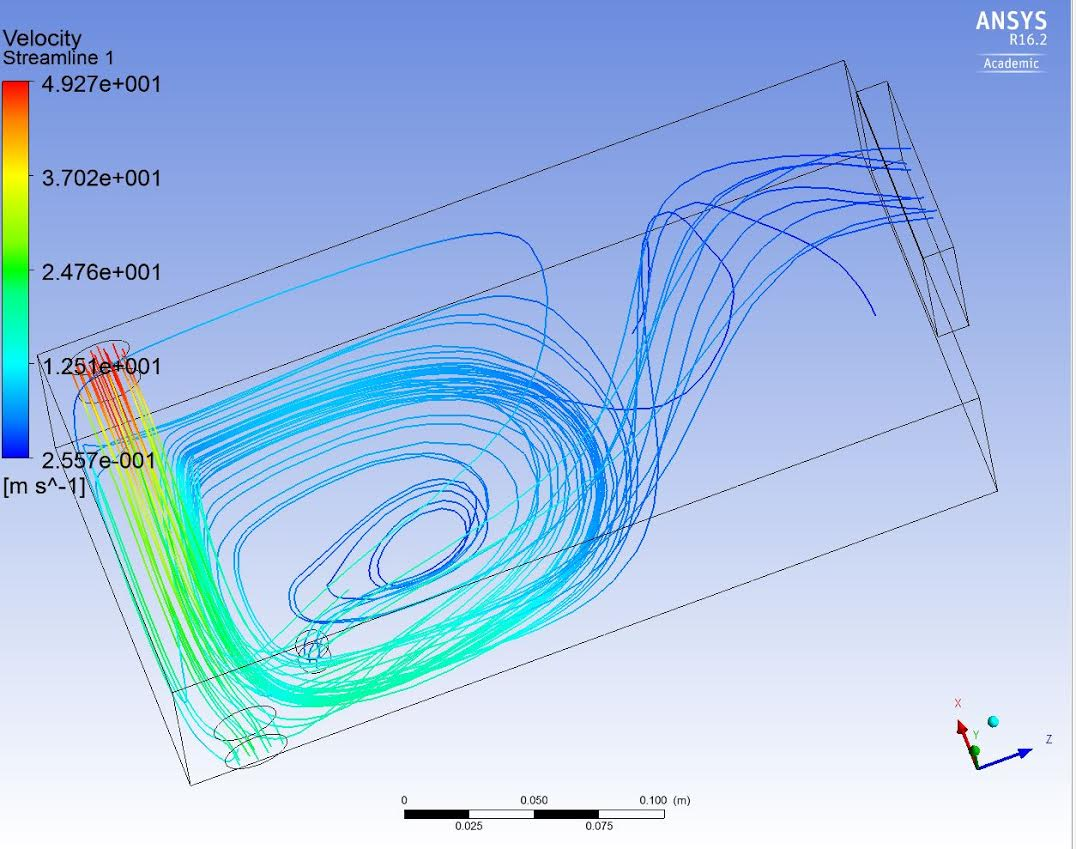
\includegraphics[scale=0.35]{CFD.jpg}
	\caption{CFD streamline analysis for our second design}
	\label{fig:CFD2}
\end{figure}

In our final iteration, we attempted to use the PWM fan as an air inlet instead, and received positive results from our CFD analysis. The use of the fan as an inlet caused the streamlines to be smooth throughout most of the system until exiting through the three outlet holes, the two primary outlets and the secondary outlet dedicated to the air particulate sensor. The streamlines showed the air exiting directly through the air particulate sensor still, while also driving air smoothly over the area where our gas sensors would be located. From this design, we built our acrylic prototypes. 

\begin{figure}[H]
	\centering
	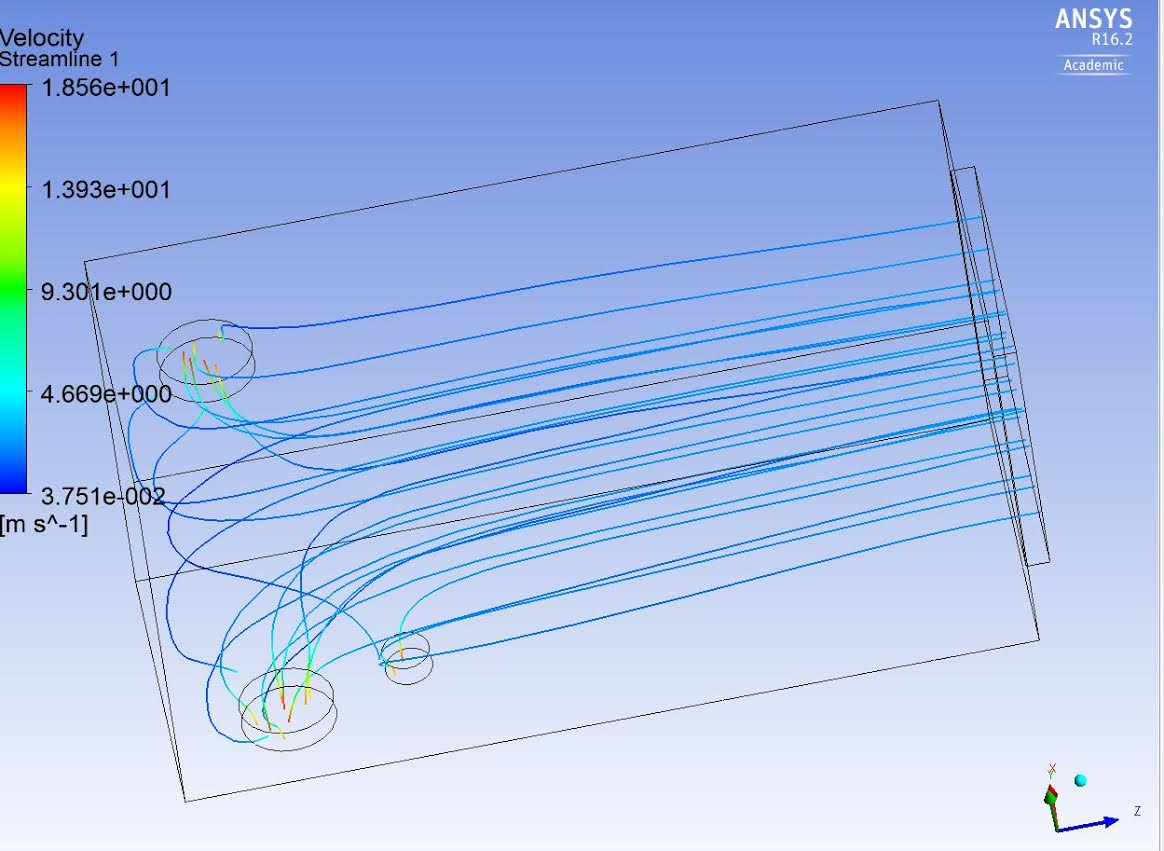
\includegraphics[scale=0.35]{CFD2.jpg}
	\caption{CFD streamline analysis for our final design}
	\label{fig:CFD}
\end{figure}

\section{Final Design}
Three housing units were made and nicknamed Larry, Curly and Moe. Each were fitted with our dedicated PCBs, which had been fitted with our gas sensors, the air particulate sensor, an Arduino unit to process the data, and the PWM fan. These fully equipped sensor units were then fitted to the roll cage of the vehicle, two, Larry and Moe, on the front cage to pull air in on both sides of the vehicle, while one, Curly, was placed at the center-front of the overhead roll cage to draw air in from the front of the vehicle. Three sensor packages were equipped onto the vehicle in such a fashion as to: protect from the case of one sensor package failing, draw air in from the three directions of concern around the vehicle, and has an aesthetically pleasing look.

\begin{figure}[H]
	\centering
	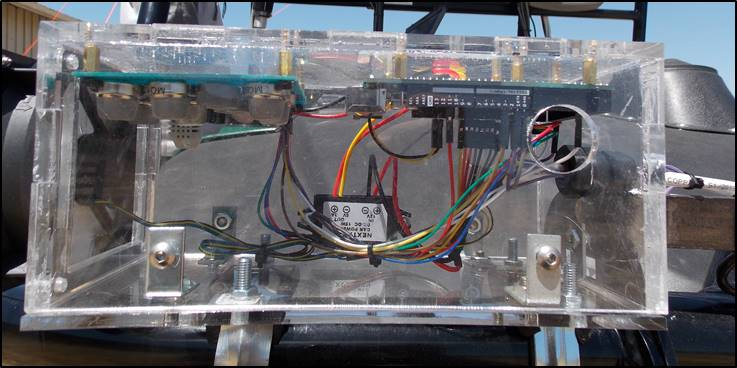
\includegraphics[scale=1.15]{SensorBox.jpg}
	\caption{The final sensor housing design equipped with our sensors, mounted to the vehicle}
	\label{fig:Box}
\end{figure}
